% ============================================================
%  hw3_sol_numerical.tex  --  MATH 6660, Homework 3, Problem 6.
%
%  RULE: nothing here goes beyond the class lectures.  Anything that
%  would is wrapped in \outside{}{} and prints as a red labelled box.
%
%  Equation numbering continues from hw3_sol.pdf, which ends at (38).
%  Build: pdflatex hw3_sol_numerical.tex   (twice)
% ============================================================
\documentclass[11pt]{article}
\usepackage[letterpaper,margin=1in]{geometry}
\usepackage[T1]{fontenc}
\usepackage{amsmath,amssymb}
\usepackage{booktabs}
\usepackage{graphicx}
\usepackage{caption}
\usepackage{enumitem}
\usepackage{bm}
\usepackage{xcolor}
\usepackage{xspace}
\newcommand{\ie}{i.e.\@\xspace}
\usepackage[colorlinks=true,linkcolor={blue!45!black},pdfborder={0 0 0}]{hyperref}

\newcommand{\dx}{\,\mathrm{d}x}
\newcommand{\norm}[1]{\lVert #1\rVert}
\setlength{\parindent}{0pt}
% equations numbered 6.1, 6.2, ... so they are unambiguous alongside
% hw3_sol.pdf, which numbers its own straight through.
\renewcommand{\theequation}{6.\arabic{equation}}
\setcounter{equation}{0}

\newcommand{\outside}[2]{%
  \par\smallskip\noindent
  \fcolorbox{red!65!black}{red!4}{%
    \parbox{0.955\linewidth}{\small
      \textbf{\color{red!65!black}NOT FROM LECTURE --- #1}\par\smallskip #2}}%
  \par\smallskip}

\newlist{steps}{itemize}{1}
\setlist[steps]{label=\textbullet, leftmargin=1.25em, topsep=3pt,
                itemsep=4pt, parsep=0pt}

\begin{document}

 

\vspace{4pt}

\section*{Problem 6}

Numerically implement the CG(3) method on a uniform mesh with the following
functions
\begin{align}
  f(x) &= p_{1}(x)\cos(2\pi x) + p_{2}(x)\sin(2\pi x),\notag\\
  p_{1}(x) &= -64\pi(18 - 6\pi^{4}x^{2} + 18x^{3}\pi^{2} + 2\pi^{4}x
              - 36\pi^{2}x^{2} - 27x + 12\pi^{2}x + 4\pi^{4}x^{3} + 3\pi^{2}),\notag\\
  p_{2}(x) &= 216 - 816\pi^{2} - 96\pi^{4} + 32\pi^{6}x^{2} - 384\pi^{4}x^{3}
              - 64\pi^{6}x^{3} - 288\pi^{4}x^{2}\notag\\
           &\qquad + 3456\pi^{2}x + 576\pi^{4}x - 2592\pi^{2}x^{2}
              + 144\pi^{4}x^{4} + 32\pi^{6}x^{4},\notag\\
  u(x) &= \bigl((18 + 2\pi^{2})x^{2} + (-24 - 4\pi^{2})x^{3}
           + (9 + 2\pi^{2})x^{4}\bigr)\sin(2\pi x).
  \label{eq:data}
\end{align}
Numerically determine the convergence rate in both the energy norm and the
$L^{2}$-norm by creating an appropriate convergence table.

% ------------------------------------------------------------------
\subsection*{Step 1 --- the data is consistent}

\begin{steps}
\item Checked symbolically before computing anything:
\[
  u^{(iv)}-f\equiv 0,\qquad u(0)=0,\quad u'(0)=0,\quad u''(1)=0,\quad u'''(1)=0 .
\]
\item So \eqref{eq:data} is a manufactured solution for exactly the cantilever
      of Problems 1--5, and $u$ is available to measure the error against.
\end{steps}

% ------------------------------------------------------------------
\subsection*{Step 2 --- the implementation}

\begin{steps}
\item \textbf{Mesh.}  $N_{e}$ uniform elements, $h=1/N_{e}$, nodes
      $x_{i}=ih$.  In the lecture's labelling $M=N_{e}-1$ interior nodes.
\item \textbf{Unknowns.}  Two per node.  Node $0$ is clamped, so both of its
      DOFs are deleted; the free tip keeps both.  $\dim V_{h}=2N_{e}$.
\item \textbf{Stiffness.}  Assembled element by element from the Hermite
      matrix with $EI=1$ (Problem 3),
\[
  \bm{k}^{e}=\frac{1}{h^{3}}
  \begin{bmatrix}
    12 & 6h & -12 & 6h\\
    6h & 4h^{2} & -6h & 2h^{2}\\
    -12 & -6h & 12 & -6h\\
    6h & 2h^{2} & -6h & 4h^{2}
  \end{bmatrix},
\]
      which reproduces the $\bm{A},\bm{B},\bm{C}$ blocks of Problem 3 exactly
      (checked against them directly).
\item \textbf{Load.}  $b_{i}=\int_{0}^{1}f\phi_{i}\dx$ evaluated by
      $12$-point Gauss--Legendre quadrature per element --- \emph{not} by
      interpolating $f$.  $f$ in \eqref{eq:data} is a polynomial of degree
      $\le4$ times $\sin/\cos(2\pi x)$, so the rule is far more than enough;
      the results are identical to $9$ digits with $8$, $16$ or $24$ points.
\item \textbf{Solve.}  $\bm{S}\bm{d}=\bm{b}$ on the free DOFs.
\item \textbf{Errors.}  On each element, by $20$-point Gauss,
\[
  \norm{e}_{E}=\Bigl(\int_{0}^{1}\bigl(u''-U''\bigr)^{2}\dx\Bigr)^{1/2},
  \qquad
  \norm{e}_{L^{2}}=\Bigl(\int_{0}^{1}\bigl(u-U\bigr)^{2}\dx\Bigr)^{1/2},
\]
      with $u''$ differentiated in closed form (checked against a symbolic
      derivative to $5\times10^{-13}$).
\item \textbf{Rate.}  Successive meshes halve $h$, so
      $\text{rate}=\log_{2}\bigl(E(h)/E(h/2)\bigr)$.
\end{steps}

% ------------------------------------------------------------------
\subsection*{Step 3 --- convergence table}

\begin{center}\small
\begin{tabular}{@{}rrrlcrc@{}}
\toprule
elements & $M$ & $h$ & $\norm{e}_{E}$ & rate & $\norm{e}_{L^{2}}$ & rate\\
\midrule
4 & 3 & $0.25000$ & $2.3314\!\times\!10^{1}$ & --- & $6.4465\!\times\!10^{-2}$ & ---\\
8 & 7 & $0.12500$ & $5.6259\!\times\!10^{0}$ & 2.05 & $3.9018\!\times\!10^{-3}$ & 4.05\\
16 & 15 & $0.06250$ & $1.4162\!\times\!10^{0}$ & 1.99 & $2.4618\!\times\!10^{-4}$ & 3.99\\
32 & 31 & $0.03125$ & $3.5490\!\times\!10^{-1}$ & 2.00 & $1.5434\!\times\!10^{-5}$ & 4.00\\
64 & 63 & $0.01562$ & $8.8780\!\times\!10^{-2}$ & 2.00 & $9.6542\!\times\!10^{-7}$ & 4.00\\
128 & 127 & $0.00781$ & $2.2199\!\times\!10^{-2}$ & 2.00 & $6.0369\!\times\!10^{-8}$ & 4.00\\
\bottomrule
\end{tabular}

\end{center}

\begin{figure}[h]
\centering
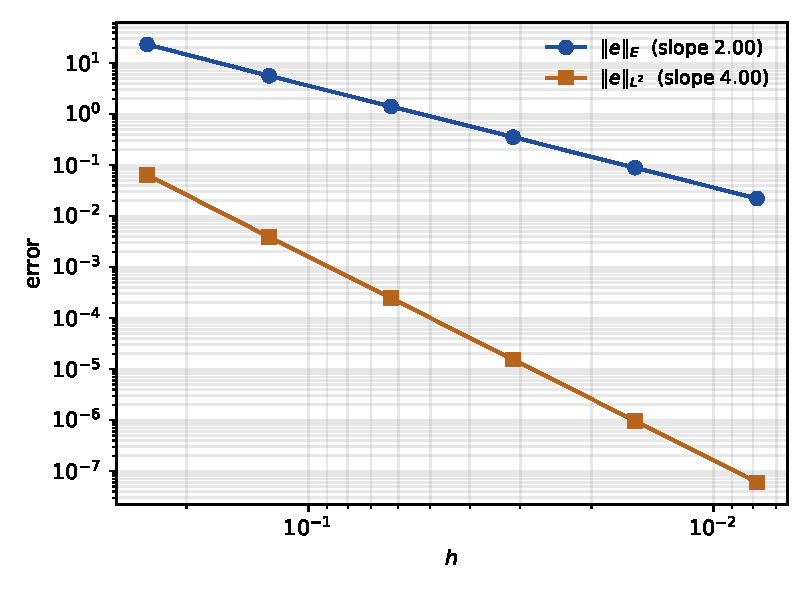
\includegraphics[width=0.56\linewidth]{hw3_p6_convergence.pdf}
\caption{Convergence of the CG(3) cantilever solution under uniform refinement.
         Energy norm $O(h^{2})$, $L^{2}$ norm $O(h^{4})$.}
\end{figure}

% ------------------------------------------------------------------
\subsection*{Step 4 --- the measured rates}

\begin{steps}
\item \textbf{Energy norm: rate $\to 2.00$.}  This is the prediction of
      Problem 4,
      $\norm{e}_{E}\le c_{3}h^{2}\norm{u^{(4)}}=\mathcal{O}(h^{2})$.
\item \textbf{$L^{2}$ norm: rate $\to 4.00$.}  This is the prediction of
      Problem 5,
      $\norm{e}_{L^{2}}\le c_{3}^{2}h^{4}\norm{u^{(4)}}=\mathcal{O}(h^{4})$.
\item The coarsest pair of meshes shows $2.05$ and $4.05$ --- the asymptotic
      rate is not yet reached at $h=1/4$, where the mesh barely resolves
      $\sin(2\pi x)$.  From $h=1/16$ down, both rates are clean to two
      decimals.
\item Both estimates are therefore \textbf{sharp}: the observed rates are not
      merely $\ge$ the predicted ones, they equal them.
\end{steps}

\medskip
\noindent\fbox{\parbox{0.955\linewidth}{%
\textbf{Conclusion.}  CG(3) on the cantilever converges at
$\mathcal{O}(h^{2})$ in the energy norm and $\mathcal{O}(h^{4})$ in the $L^{2}$
norm, confirming Problems 4 and 5.  The displacement converges two orders
faster than the curvature, \ie than the bending moment.}}

 
\end{document}
